\documentclass[]{article}

\usepackage[margin=1.0in]{geometry}
\usepackage{amsmath}
\usepackage{amsfonts}
\usepackage{amsthm}
\usepackage{graphicx}
\usepackage{amssymb}

\usepackage{mathtools}

%opening
\title{Schottky Group Example}
\author{Alex Karlovitz}
\date{}

\begin{document}
	
	\maketitle
	
\section*{Schottky Groups in the Unit Disk}

We can form a Schottky group in the unit disk as follows:
let $\mathcal{C}$ be a finite collection of disjoint circles which are orthogonal to the unit circle (actually, we will allow two circles in $\mathcal{C}$ to be tangent, so their intersections with the open unit disk are disjoint).
Then the group $\Gamma(\mathcal{C})$ generated by reflections across these circles in the unit disk is an example of a \textit{Schottky group}.

\subsection*{Example: Symmetric Circles}

A simple example of a Schottky group in the unit disk is obtained by taking circles of the same size spaced symmetrically about the disk.
We could parameterize such sets of circles by the two variables $n$ and $\theta$, where $n$ is the number of circles and $\theta$ is the angle along the unit circle cut out by one of the circles.
See Figure \ref{pi_over_2} for an example.

\begin{figure}[h]
	\centering
	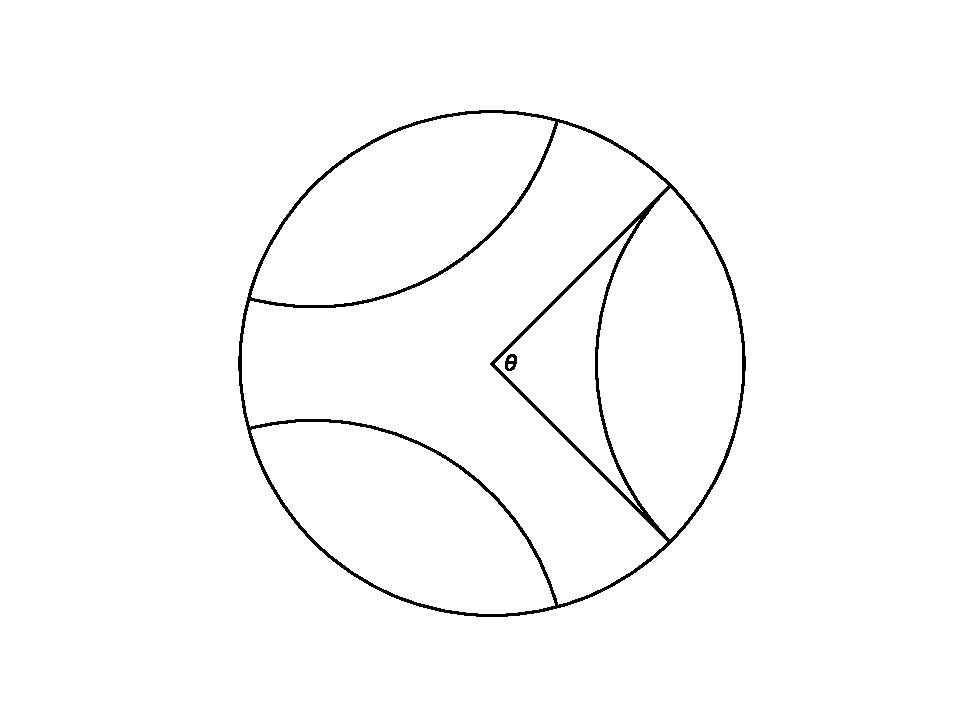
\includegraphics[trim=110 40 100 50, clip, width=0.6\linewidth]{pi_over_2.pdf}
	\caption{Example with $n = 3$ circles cutting out arcs of angle $\theta = \frac{\pi}{2}$}
	\label{pi_over_2}
\end{figure}

A fundamental domain for such a Schottky group is the exterior of all the circles (inside the unit disk of course).
To see this, label the reflections across the $n$ circles $R_1, \dots, R_n$.
We will also use $R_i$ to denote the actual reflections; the meaning should be clear from context.
Let
$$
\gamma = R_{i_1}\cdots R_{i_k}
$$
be a reduced word of length $k$ in the reflections (by \textit{reduced} we mean that $R_{i_j} \neq R_{i_{j+1}}$ for all $j$, since reflections are involutions).
Note that every element of the Schottky group can be written as such a reduced word.
Now suppose $z$ is any element of the fundamental domain.
If $k = 1$, then it is clear that $\gamma(z)$ is inside the circle $R_{i_1}$.
By induction, it is then easy to see that for $k \geq 1$, $\gamma(z)$ is always in the circle $R_{i_1}$.
Thus, the only way for $\gamma(z)$ to be in the fundamental domain is t o have $k = 0$; i.e., $\gamma$ is the identity.

To see that every orbit has a point in the fundamental domain, one must check that given a point in one of the circles $R_i$, reflection through that circle \textit{decreases} the distance from the point to $0$.
Thus, since the Schottky group acts discretely on hyperbolic space, we can eventually move any point to the fundamental domain by repeatedly reflecting outside of any circle it falls in.

See Figure \ref{disk_FD} for an example.

\begin{figure}[h]
	\centering
	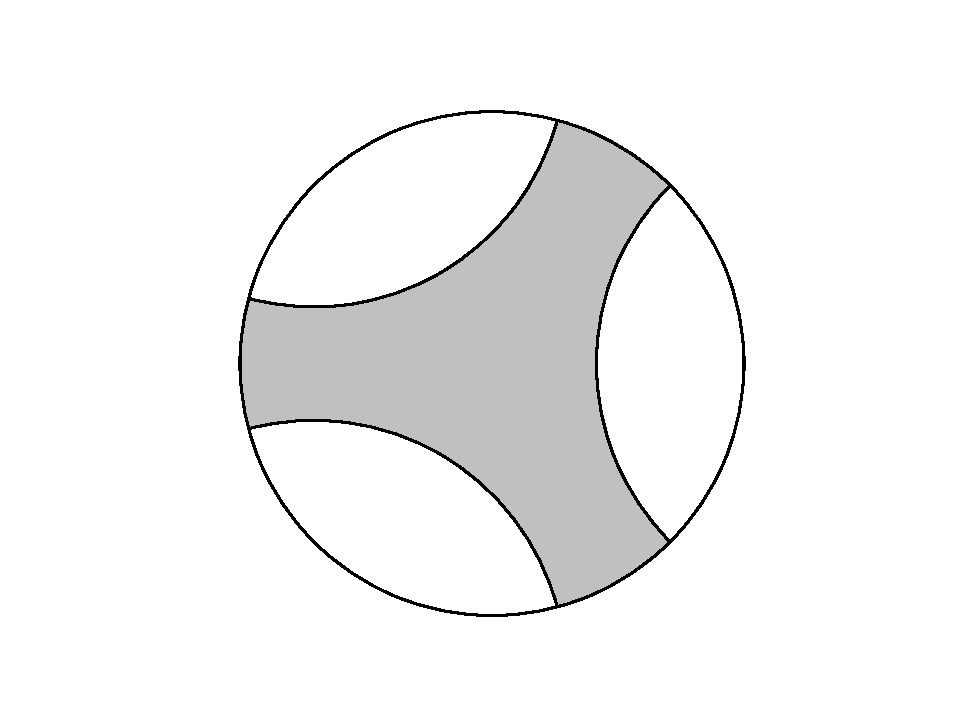
\includegraphics[trim=110 40 100 50, clip, width=0.6\linewidth]{disk_FD.pdf}
	\caption{The example from Figure \ref{pi_over_2} with a fundamental domain filled in.}
	\label{disk_FD}
\end{figure}

\section*{Taking our Schottky Groups to the Upper Half Plane}

Recall that we can map from the upper half plane model to the disk model via the \textit{Cayley transform}
$$
C(z) = \frac{z - i}{z + i}
$$
We can go the other direction by taking the inverse
$$
C^{-1}(w) = i\cdot\frac{1 + w}{1 - w}
$$
Also recall that $C$ and $C^{-1}$ send geodesics to geodesics.

Next, note that we are choosing to center one of our circles of reflection about $1$.
Since $C^{-1}(1) = \infty$, this has the effect of forcing our fundamental domain to be bounded inside $C^{-1}$ of that circle.
See Figure \ref{UHP_FD} for an example.

\begin{figure}[h]
	\centering
	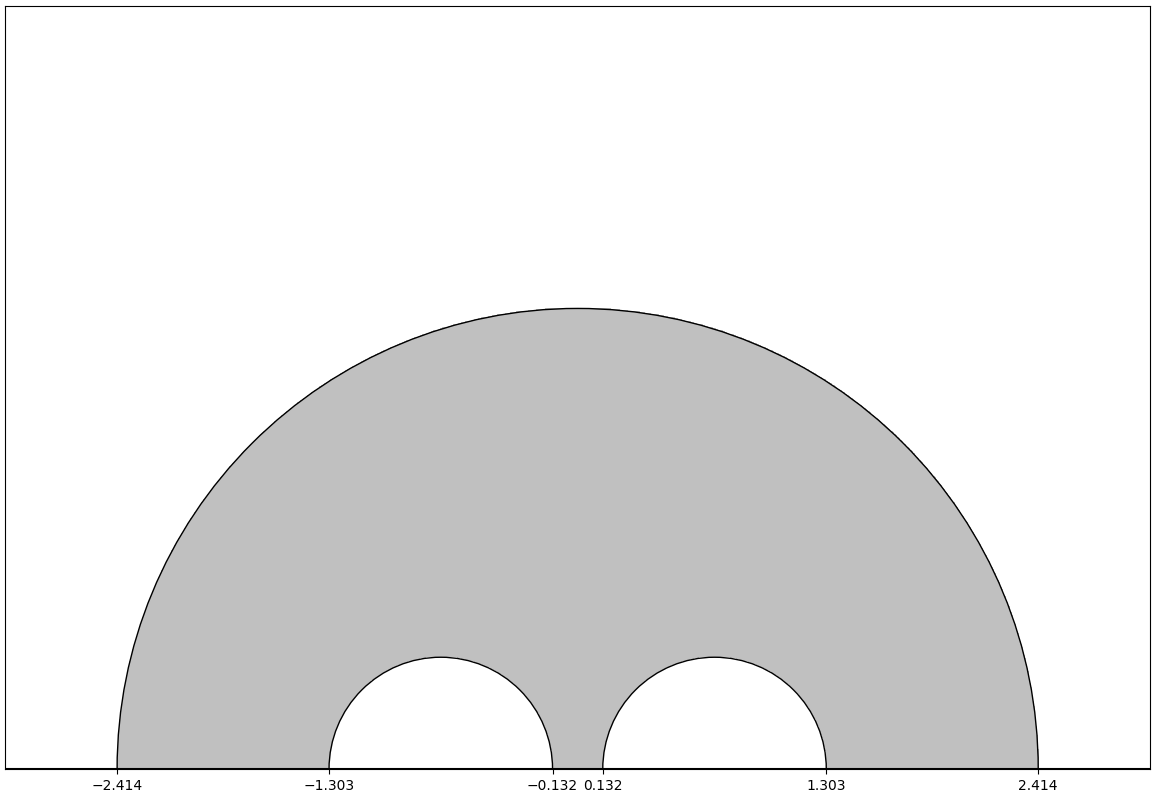
\includegraphics[width=0.8\linewidth]{UHP_FD.png}
	\caption{The example from the previous section ($n = 3, \theta = \frac{\pi}{2}$) mapped to the upper half plane.}
	\label{UHP_FD}
\end{figure}

\subsection*{Doubling Across a Reflection}

Next, note that reflections are \textit{not} M\"obius transformations.
Instead, they are compositions of M\"obius transformations with reflections across vertical lines.
Since we would like to work with M\"obius transformations (so that our maps can be realized as elements of $\text{SL}(2, \mathbb{R})$), we will pass to a double cover of the Schottky group.
This is achieved by \textit{doubling} across one of the reflections.
\\

We begin as before with the Schottky group generated by the $n$ reflections $R_1, \dots, R_n$.
We then single out one of the reflections, say $R_1$, and consider the group generated by the rest of the reflections \textit{composed with} $R_1$.
That is, we look at
$$
\Gamma = \langle R_1R_2, \dots, R_1R_n \rangle
$$
By composing two circle reflections, the two vertical reflections cancel out, and we are left with a M\"obius transformation.
Therefore, $\Gamma \subseteq \text{SL}(2, \mathbb{R})$.
\\

A fundamental domain for this group is obtained by reflecting the previous fundamental domain across $R_1$.
See Figure \ref{doubled_FD} for an example.

\begin{figure}[h]
	\centering
	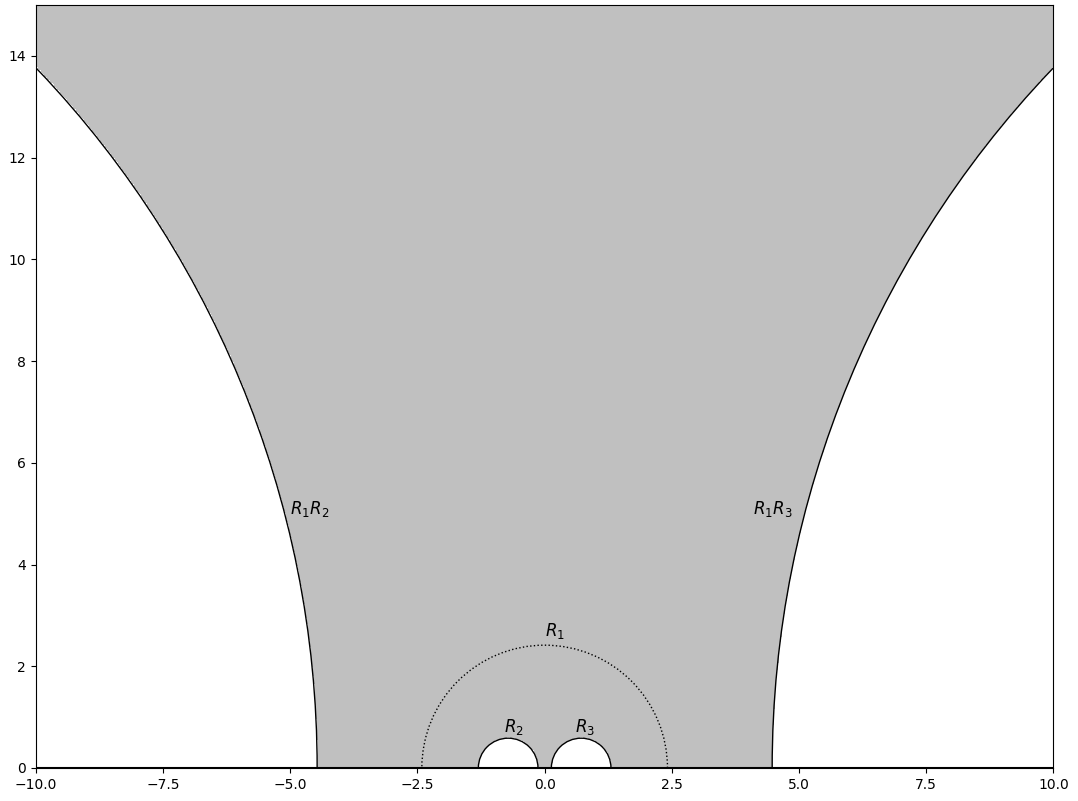
\includegraphics[width=\linewidth]{doubled_FD.png}
	\caption{The $n = 3$, $\theta = \frac{\pi}{2}$ example, doubled.}
	\label{doubled_FD}
\end{figure}

\subsection*{Identifying Flare Domains}

To get a flare domain, we need to identify a hyperbolic element in our group of M\"obius transformations whose axis\footnote{Recall that the \textit{axis} of a hyperbolic matrix is the geodesic whose endpoints are the fixed points of the matrix.} ``cuts off'' a flare in our fundamental domain.
To do this, we need to look at a specific example.
Let us start with the case of the symmetric Schottky groups defined above, say with 3 circles.
\\

After mapping to the upper half plane and doubling across $R_1$, our group of M\"obius transformations will look like
$$
\Gamma = \langle R_1R_2, R_1R_3 \rangle
$$
See Figure \ref{doubled_FD} for the fundamental domain.
At first glance, we appear to have four flares:
\begin{itemize}
	\item one between circles $R_1R_2$ and $R_2$
	\item one between $R_2$ and $R_3$
	\item one between $R_3$ and $R_1R_3$
	\item and one ``at infinity''
\end{itemize}
Note that the flare ``at infinity'' can be thought of as a flare between circles $R_1R_2$ and $R_1R_3$.
This is most easily visualized in the disk model.
\\

To identify a flare between geodesics $C_1$ and $C_2$, one may look for a geodesic with the following properties:
\begin{itemize}
	\item one endpoint of the geodesic is on the other side of $C_1$ from the flare
	\item the other endpoint is on the other side of $C_2$ from the flare
	\item the geodesic meets $C_1$ and $C_2$ at right angles
\end{itemize}
In our situation, it is always possible to find a hyperbolic element in $\Gamma$ whose axis satisfies these properties.
To see this, one looks in inversive coordinates (see Kontorovich's letter to Bill Duke).
Letting $v_1$ and $v_2$ denote the inversive coordinates for $C_1$ and $C_2$, respectively, one looks for the inversive coordinates $v$ such that
$$
v_1^tQv = 0 ~~~~~ v_2^tQv = 0 ~~~~~ v^tQv = -1
$$
where $Q$ is the quadratic form defining inversive coordinates.
The first two equations give the orthogonality, and the third gives a true vector of inversive coordinates.
Finally, these coordinates give the endpoints of our geodesic.
To find the corresponding M\"obius transformation in $\Gamma$, one searches over all transformations with this axis for the one taking the intersection point with $C_1$ to that of $C_2$.
\\

Instead of utilizing the robust process just described, one finds the hyperbolic elements in $\Gamma$ whose axes cut off the flares by looking at small words in the generators.
This quickly leads to three of the four matrices:
\begin{itemize}
	\item between $R_2$ and $R_3$: $(R_1R_2)^{-1}R_1R_3 = R_2R_3$
	\item between $R_1R_2$ and $R_2$: $R_1R_2$
	\item between $R_1R_3$ and $R_3$: $R_1R_3$
	\item between $R_1R_2$ and $R_1R_3$: letting $C$ be the axis for $R_2R_3$, the geodesic $R_1(C)$ cuts off this flare
\end{itemize}
There is a very good reason one of these flares appears to behave differently from the other three.
In fact, the flare between $R_1R_2$ and $R_1R_3$ is actually \textit{part of} the flare between $R_2$ and $R_3$.
To see this, note that the M\"obius transformation $R_1R_3$ takes $C$ to $R_1(C)$.
In other words, $C$ is not itself a closed geodesic; instead, $C$ and $R_1(C)$ together form a closed geodesic.
We will rectify this issue in a moment.

For now, we verify the above results computationally in python, and this produces the image in Figure \ref{flares}.
\begin{figure}[h]
	\centering
	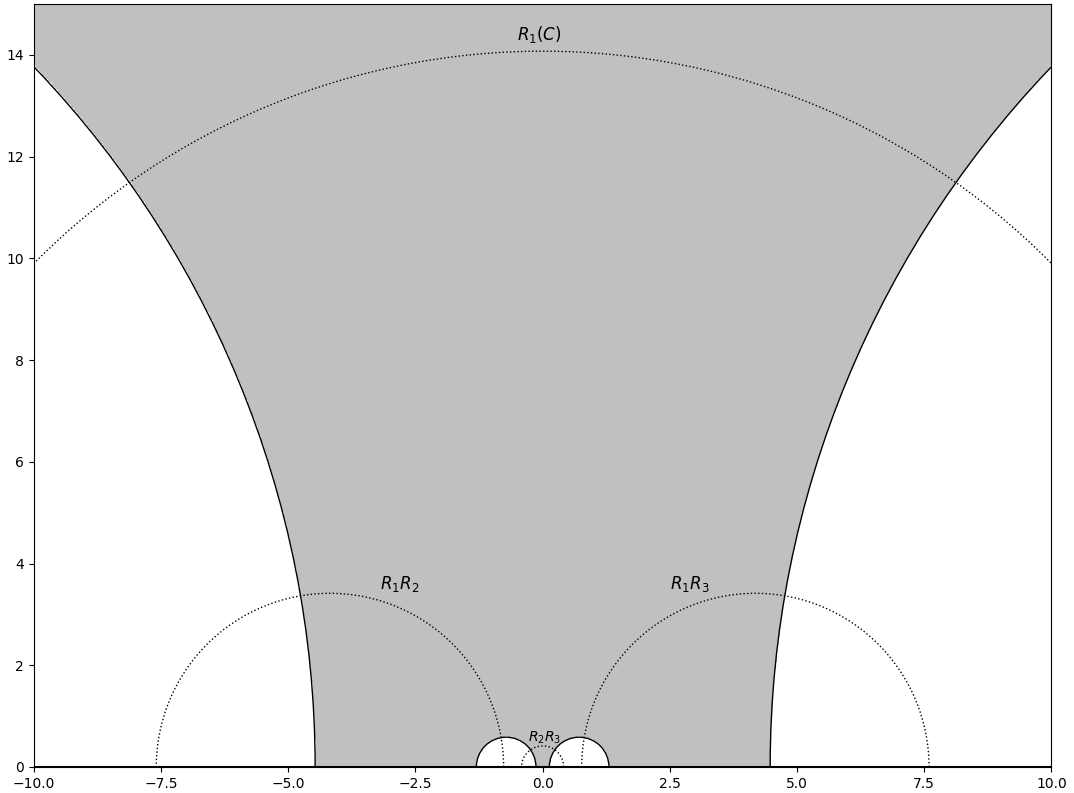
\includegraphics[width=\linewidth]{flares.png}
	\caption{Doubled example with flares drawn $(n = 3$, $\theta = \frac{\pi}{2})$.}
	\label{flares}
\end{figure}
See the code in schottkyGroups.py.
This verification relies on some of the computations in the appendix.

\clearpage

\subsection*{Combining Equivalent Flares}

As discussed in the previous section, the natural fundamental domain of a Schottky group - after doubling across one of the circles in the upper half plane model - could have a flare which ``split'' into multiple pieces.
To rectify this, one simply applies group transformations to disjoint subsets of the fundamental domain to move split flares next to each other.
We illustrate this with an example.

Let us return again to the symmetric Schottky group with parameters $n = 3, \theta = \frac{\pi}{2}$.
We will denote the natural fundamental domain (as seen in Figures \ref{doubled_FD} and \ref{flares}) $\mathcal{F}$.
Consider the following breakdown of $\mathcal{F}$ into disjoint subsets
$$
\mathcal{F} = \mathcal{F}_1 \cup \mathcal{F}_2 \cup \mathcal{F}_3
$$
where
$$
\mathcal{F}_1 = \mathcal{F} \cap \overline{\text{ext}(R_1)} \cap \text{Im}(z) < 0, ~~~
\mathcal{F}_2 = \mathcal{F} \cap \overline{\text{ext}(R_1)} \cap \text{Im}(z) >= 0, ~~~
\mathcal{F}_3 = \mathcal{F} \cap \text{int}(R_1)
$$
See Figure \ref{disjoint_FD} for a visual.
\begin{figure}[h]
	\centering
	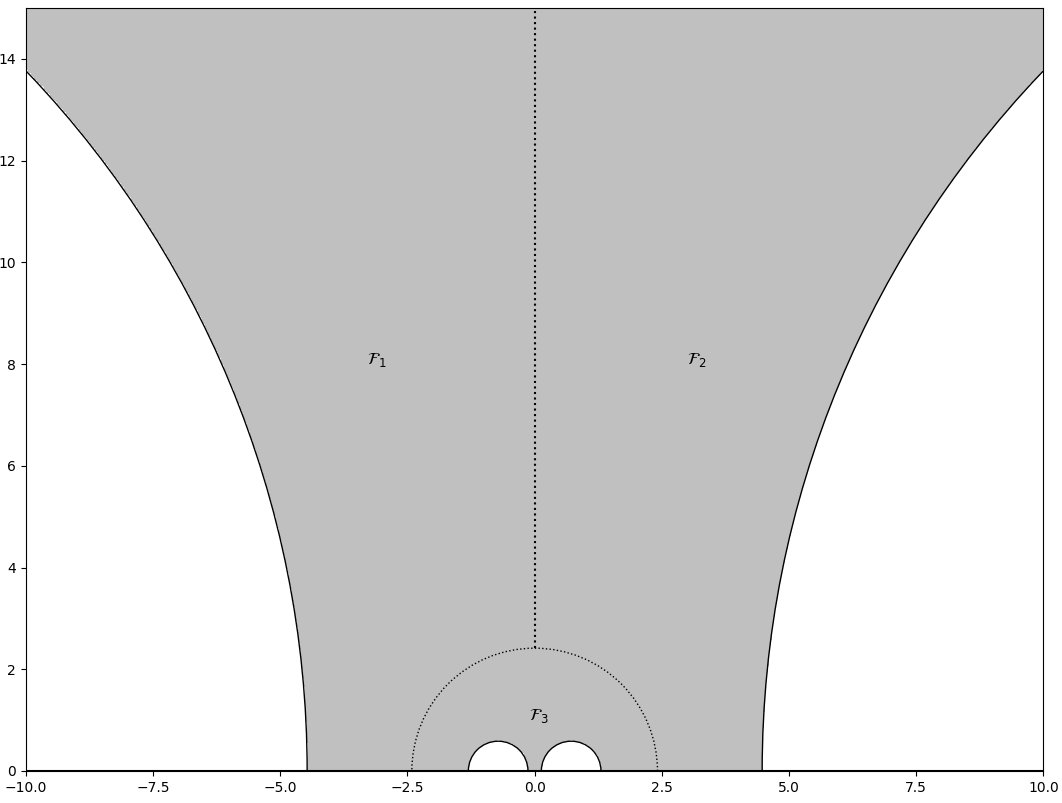
\includegraphics[width=\linewidth]{disjoint_FD.png}
	\caption{Fundamental domain split into disjoint sets, pre-mapping.}
	\label{disjoint_FD}
\end{figure}

Next, we map over to a new fundamental domain
$$
\hat{\mathcal{F}} = R_2R_1(\mathcal{F}_1) \cup R_3R_1(\mathcal{F}_2) \cup \mathcal{F}_3
$$
This has the effect of taking $\mathcal{F}_1$ inside the circle $R_2$ and $\mathcal{F}_2$ inside $R_3$.
See Figure \ref{shifted_FD} for a visual.
\begin{figure}[h]
	\centering
	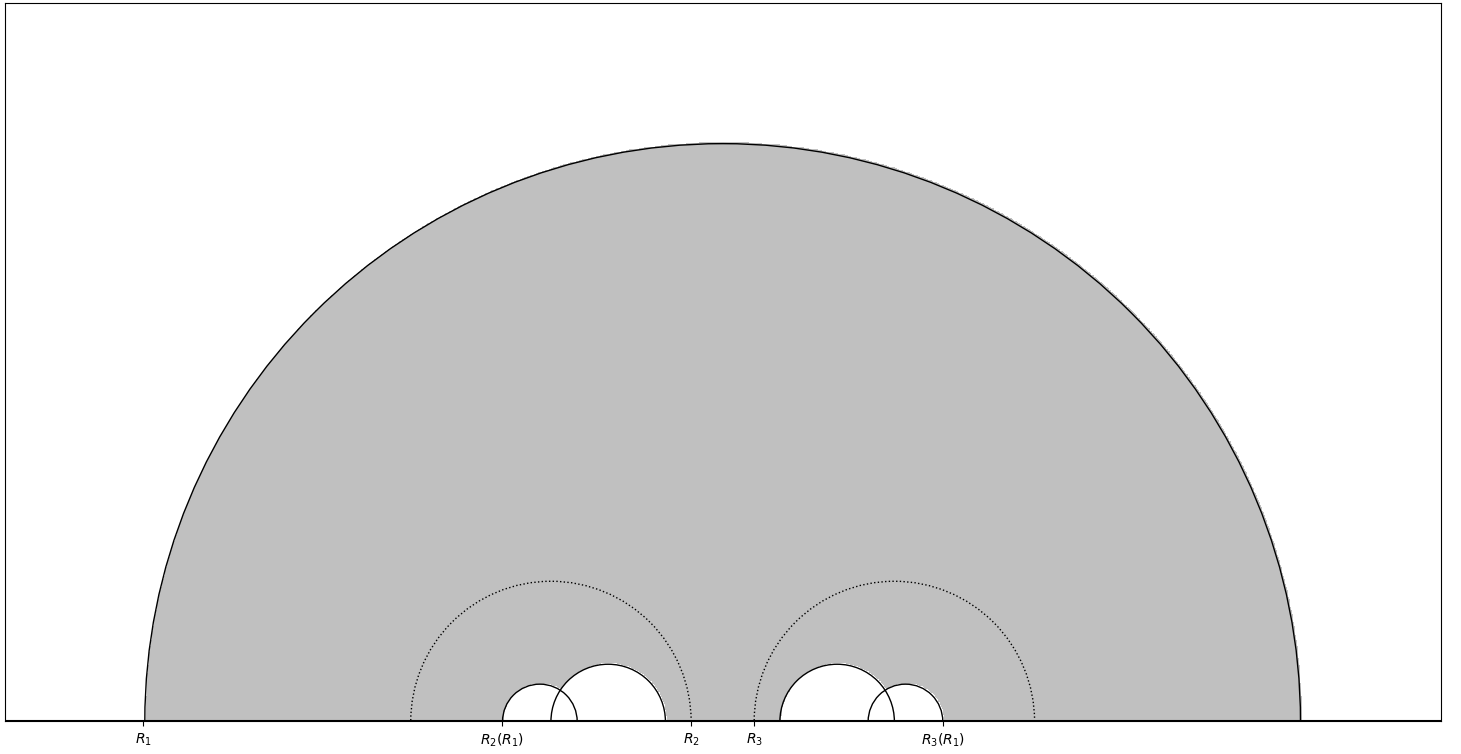
\includegraphics[width=0.9\linewidth]{shifted_FD.png}
	\caption{Fundamental domain split into disjoint sets, post-mapping.}
	\label{shifted_FD}
\end{figure}

Finally, we note that the same geodesics which cut off the flares before (shown in Figure \ref{flares}) will still cut off the appropriate flares here.
For example, note that the geodesic whose endpoints are fixed by $R_3R_1$ is also the axis of $R_1R_3$ (since $R_1R_3 = (R_3R_1)^{-1}$).
Thus, mapping geodesics by $R_3R_1$ preserves the angle of intersection with this geodesic.
See Figure \ref{shifted_with_flares} for our new fundamental domain with the flares drawn.
\begin{figure}[h]
	\centering
	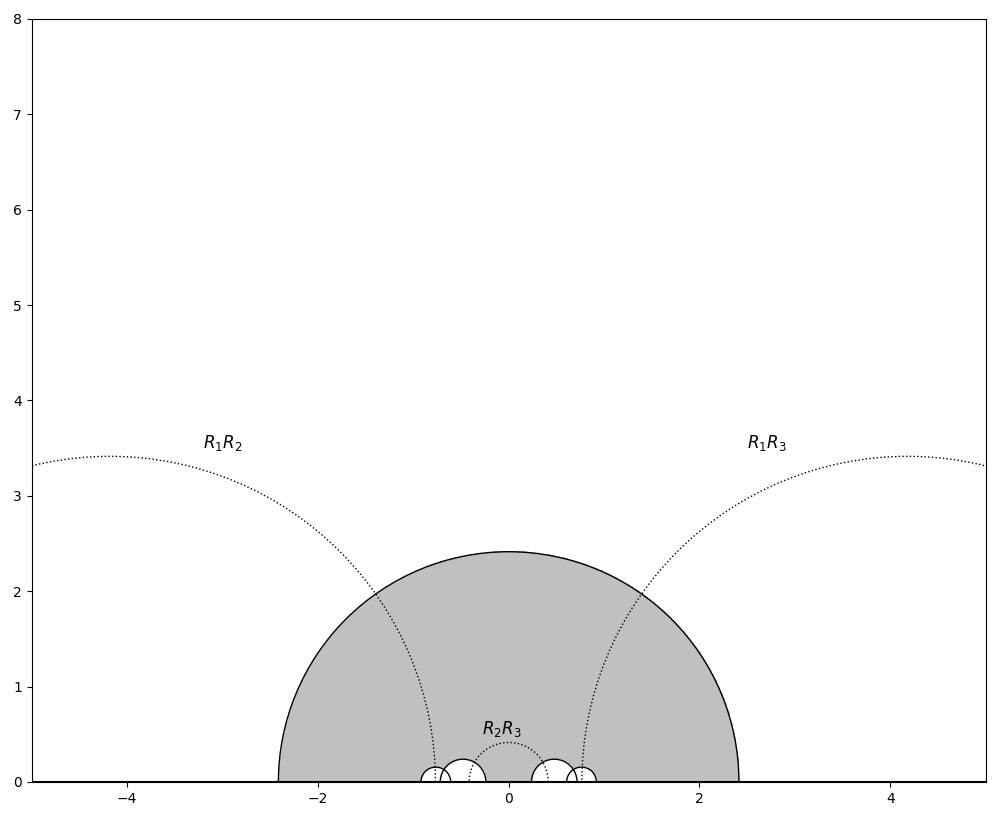
\includegraphics[width=0.9\linewidth]{shifted_with_flares.png}
	\caption{New fundamental domain with three flares.}
	\label{shifted_with_flares}
\end{figure}

\clearpage

\subsection*{Mapping to a Flare Domain}

Let us look at a generic flare: two geodesics separated by positive length interval on the real line, plus a geodesic cutting through both of these at a right angle.
Let the two points on this last geodesic be labeled $z_1 < z_2$, and call the rightmost point of the first geodesic $t$.
See Figure \ref{pre_flare}.
\begin{figure}[h]
	\centering
	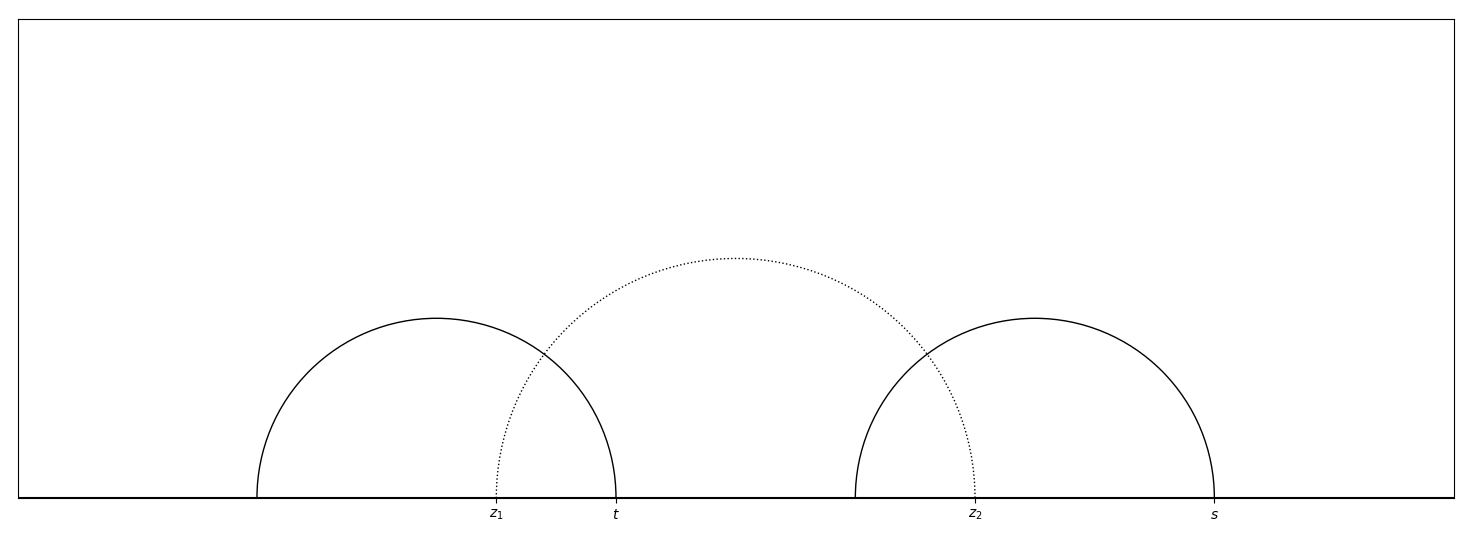
\includegraphics[width=\linewidth]{labeled_pre_flare.png}
	\caption{A generic flare.}
	\label{pre_flare}
\end{figure}
Now consider the M\"obius transformation
$$
U(z) = \left( \frac{t - z_2}{t - z_1} \right) \frac{z - z_1}{z - z_2}
$$
This function is chosen so that
$$
U(z_1) = 0 ~~~~~ U(z_2) = \infty ~~~~~ U(t) = 1
$$
Thus, applying such a $U$ to a generic flare gives us a \textit{flare domain}.
See Figure \ref{post_flare} for an example.
\begin{figure}[h]
	\centering
	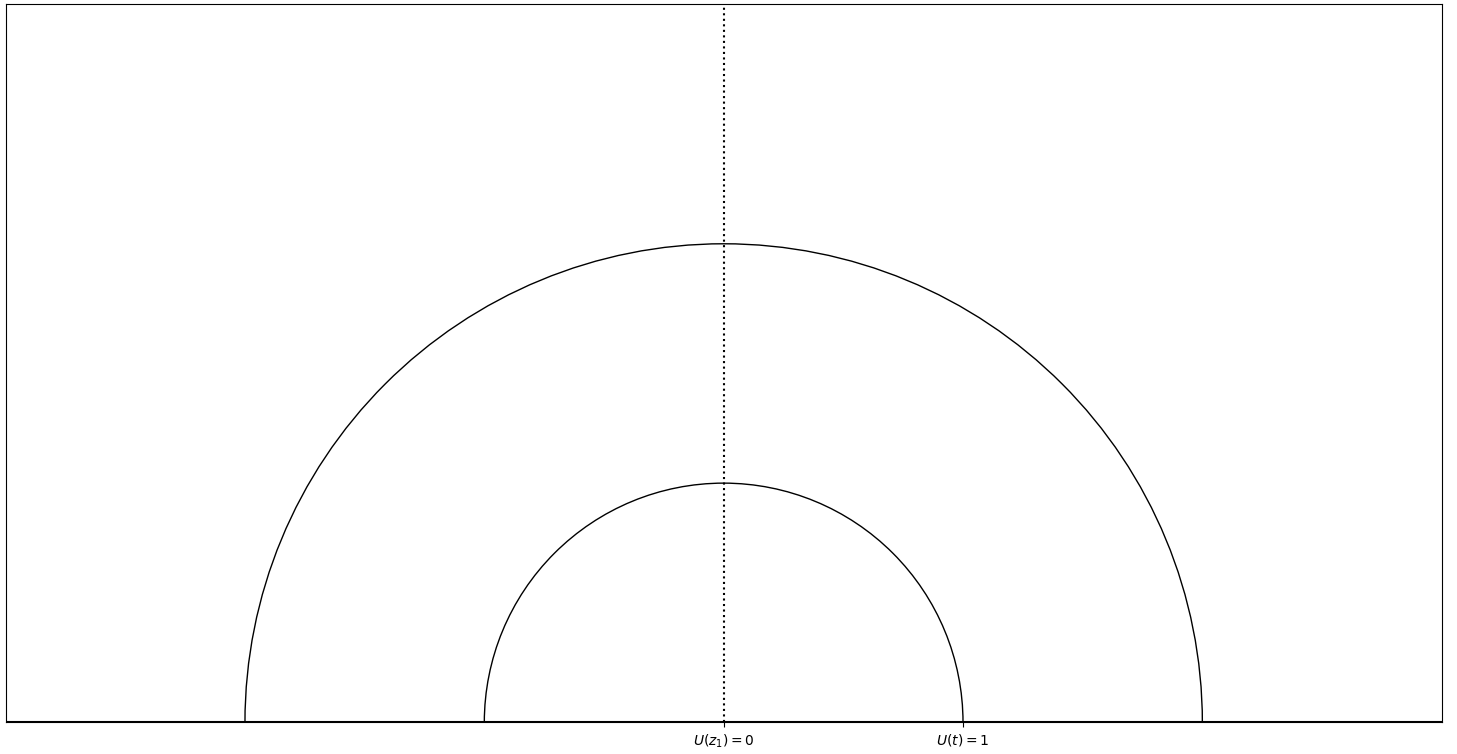
\includegraphics[width=\linewidth]{labeled_flare.png}
	\caption{A flare domain.}
	\label{post_flare}
\end{figure}

We now return to our example from before (the Schottky group with $n = 3$ and $\theta = \frac{\pi}{2}$).
Since we have the endpoints of all the geodesics involved, we can map each flare to a flare domain.
It is in such flare domains where we will take Fourier expansions in polar coordinates for Hejhal's algorithm.
See Figures \ref{flare_R1R2} - \ref{flare_R2R3} for these images.
Again, the code producing the figures can be found in schottkyGroups.py.
\begin{figure}[h]
	\centering
	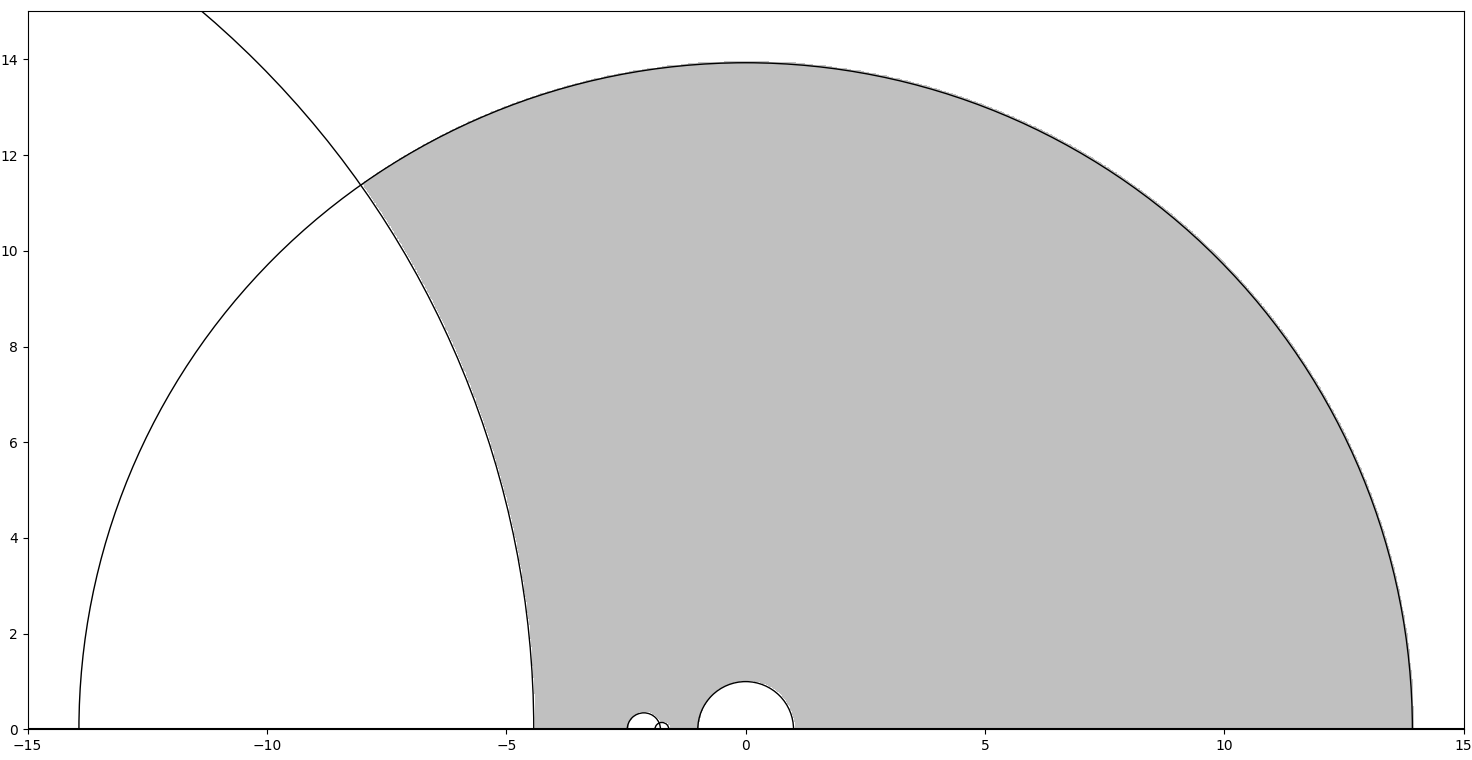
\includegraphics[width=\linewidth]{flare_R1R2.png}
	\caption{Flare domain from flare with axis $R_1R_2$.}
	\label{flare_R1R2}
\end{figure}
\begin{figure}[h]
	\centering
	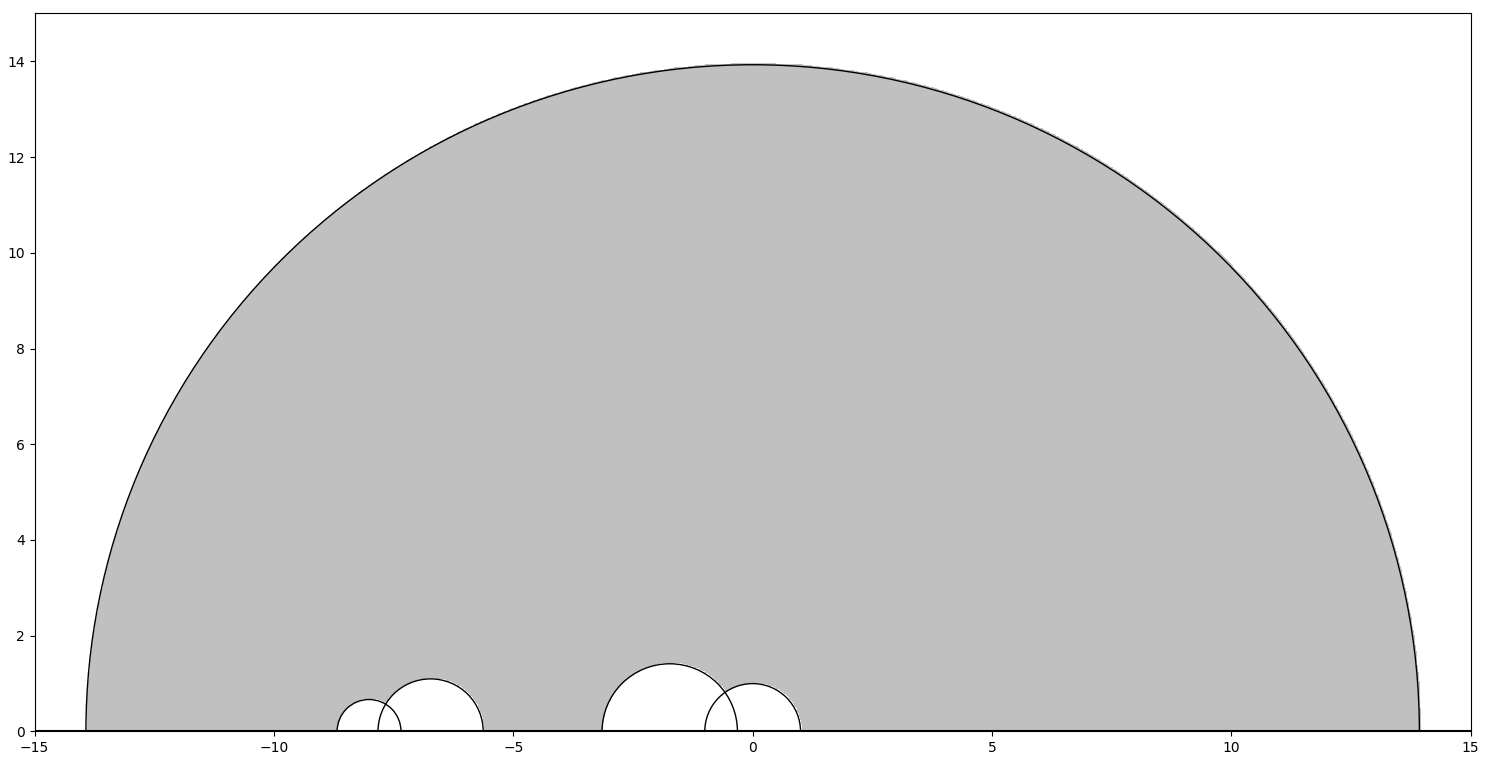
\includegraphics[width=\linewidth]{flare_R1R3.png}
	\caption{Flare domain from flare with axis $R_1R_3$.}
	\label{flare_R1R3}
\end{figure}
\begin{figure}[h]
	\centering
	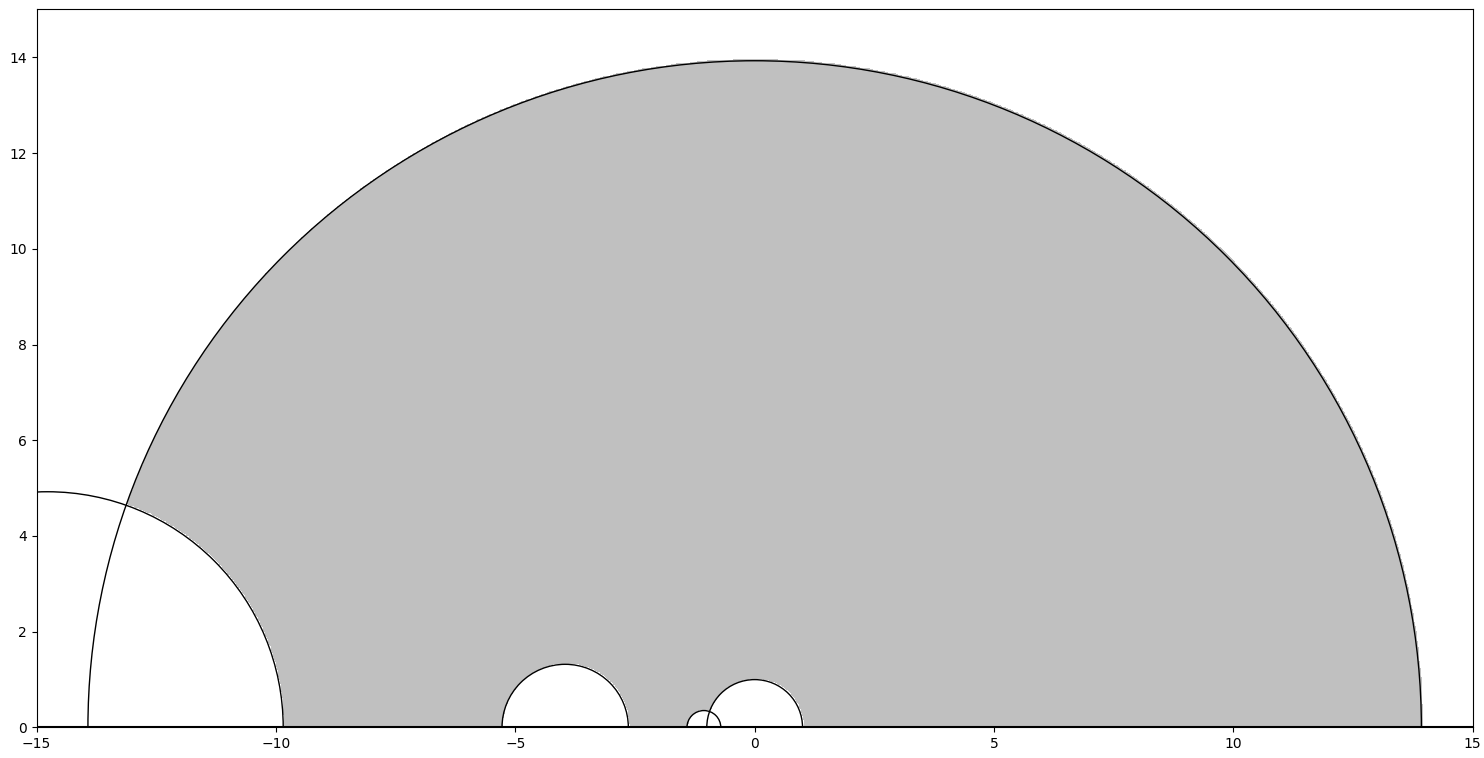
\includegraphics[width=\linewidth]{flare_R2R3.png}
	\caption{Flare domain from flare with axis $R_2R_3$.}
	\label{flare_R2R3}
\end{figure}

\clearpage

\section*{Appendix: Computations with M\"obius Transformations and Reflections}

Recall that the M\"obius transformation
$$
S_r(z) = \frac{-r^2}{z}
$$
acts by reflecting across the circle of radius $r$ centered at the origin followed by reflection across the imaginary axis.
Let us denote reflection across the circle of radius $r$ centered at $c$ by $C_{r, c}$ and reflection across the vertical line $\text{Re}(z) = c$ by $R_c$.
Then the previous claim may be written as
$$
S_r(z) = R_0\circ C_{r, 0}(z) = C_{r, 0}\circ R_0(z)
$$
(Note that these two reflections commute).
We could center this action at any point $c \in \mathbb{R}$ by shifting to the origin, applying $S_r$, then shifting back.
That is, if we define $S_{r, c} := R_c \circ C_{r, c} = C_{r, c}\circ R_c$, then
$$
S_{r, c}(z) = S_r(z - c) + c = \frac{-r^2}{z - c} + c
$$

Now, note that $S_{r, c}$ is a M\"obius transformation, since
$$
S_{r, c}(z) = \frac{cz - (r^2 + c^2)}{z - c} =
\begin{pmatrix}
	c & -(r^2 + c^2) \\
	1 & -c
\end{pmatrix}(z)
$$
Thus, since reflections are involutions, we have that $C_{r, c} = S_{r, c}\circ R_c = R_c\circ S_{r, c}$ is the composition of a M\"obius transformation with reflection across a vertical line (as claimed above).
We furthermore claimed that the \textit{composition} of reflections across two circles is M\"obius.
To see this, we first note that a composition of reflections across vertical lines is M\"obius.
Since
$$
R_c(z) = z - 2(\text{Re}(z) - c) = 2c - \bar{z},
$$
we have that
$$
R_c\circ R_a(z) = z + 2(c - a) =
\begin{pmatrix}
	1 & 2(c - a) \\
	0 & 1
\end{pmatrix}(z)
$$
Finally, we compute the composition of circle reflections:
$$
C_{r, c}\circ C_{t, a}(z) = S_{r, c}\circ R_c\circ R_a\circ S_{t, a}(z) = $$$$
\begin{pmatrix}
c & -(r^2 + c^2) \\
1 & -c
\end{pmatrix}
\begin{pmatrix}
1 & 2(c - a) \\
0 & 1
\end{pmatrix}
\begin{pmatrix}
a & -(t^2 + a^2) \\
1 & -a
\end{pmatrix}(z) $$$$ =
\begin{pmatrix}
c^2 - ac - r^2 & a^2c - ac^2 + ar^2 - ct^2 \\
c - a & a^2 - ac - t^2
\end{pmatrix}(z)
$$
Let us denote this final matrix $M_{(r, c), (t, a)}$.
Note that it has determinant $r^2t^2 \neq 0$.
Therefore, the matrix $A := A_{(r, c), (t, a)} = \frac{1}{rt}M_{(r, c), (t, a)}$ defines the same M\"obius transformation and has $A \in \text{SL}(2, \mathbb{R})$.

Finally, recall that the matrix $
\left(
\begin{smallmatrix}
a & b \\
c & d
\end{smallmatrix}
\right) \in \text{SL}(2, \mathbb{R})$ has fixed points
$$
\frac{a - d \pm \sqrt{(a + d)^2 - 4}}{2c}
$$
Therefore, the fixed points of our M\"obius transformation $C_{r, c}\circ C_{t, a}$ are
$$
\frac{c^2 - a^2 + t^2 - r^2 \pm \sqrt{( (a - c)^2 - (r^2 + t^2) )^2 - 4r^2t^2}}{2(c - a)}
$$

\section*{Appendix: Considerations for Hejhal's Algorithm}

Consider Figure \ref{shifted_with_flares} once more, where we picture our final fundamental domain along with its flares.
Suppose we take a point $z$ which lies \textit{inside} the flare defined by $R_1R_3$ but \textit{outside} the fundamental domain.
We claim that the pullback of $z$ to the fundamental domain is obtained by applying $(R_1R_3)^n$ for some $n \in \mathbb{Z}$, $n \neq 0$.
This can be seen geometrically by recalling that a hyperbolic transformation ``slides points'' along its axis.
Points inside the axis or outside the axis slide in a similar manner, remaining on their side of the geodesic.

Next, let's consider this same action in the corresponding flare domain.
Note that the main purpose of mapping to the flare domain is to convert the hyperbolic transformation into a scaling matrix (of course, this is still a hyperbolic transformation; just a very specific and simple one).
Specifically, the action is converted to one of the form
$$
z \mapsto \kappa z
$$
for some $\kappa > 1$.
So the pullback is equal to $\kappa^nz$ for some $n \in \mathbb{Z}, n \neq 0$.
Furthermore, recall that it is this action which leads to a logarithmic Fourier expansion of Maass forms.
Specifically, if $\phi$ is a Maass form for such a Schottky group, where $\phi(r, \theta)$ is a function of the polar coordinates $(r, \theta)$ in the flare, then
$$
\phi(r, \theta) = \sum_{n\in\mathbb{Z}}g_n(\theta)e\left( n\frac{\log r}{\log \kappa} \right)
$$
But note that $\phi(r, \theta)$ is then automatically invariant under the map $z \mapsto \kappa z$.
Thus, we gain \textit{no new information} by taking such a test point $z$.
\\

\textbf{Conclusion:} for Hejhal's algorithm, we should not use test points inside a flare but outside the fundamental domain.
For in this case, the algorithm would attempt to compare the flare expansion at the test point to the same expansion at its pullback, but this garners no new information.

\subsection*{Hausdorff Dimension}

McMullen's program ``hdim'' (available on his website) computes the Hausdorff dimension of the limit sets of the symmetric Schottky groups described in this note (as well as a variety of other types of ``Kleinian group[s] generated by reflections in the boundaries of a family of \textit{disjoint} round disks in the plane'').
In our notation for Hejhal's algorithm, we deal with the Hausdorff dimension $s$, which is related to the eigenvalue $\lambda$ via the equation
$$
\lambda = s(1 - s)
$$
Here we list some $s$ values for the symmetric Schottky groups with 3 circles of angle $\theta$ for various $\theta$.
\begin{center}
	\begin{tabular}{c|c}
		$\theta$ & $s$ \\
		\hline
		$\pi/6$ & 0.18398306 \\
		$\pi/3$ & 0.29554650 \\
		$\pi/2$ & 0.47218812
	\end{tabular}
\end{center}

\end{document}